\documentclass{article}
\usepackage[utf8]{inputenc}
\usepackage{listings}
\usepackage{float}
\usepackage{natbib}
\usepackage{graphicx}
\usepackage{amssymb}
\usepackage{amsmath}
\usepackage{mathtools}
\usepackage{listings}
\usepackage{color}
\usepackage{hyperref}
\usepackage{ amssymb }

\definecolor{dkgreen}{rgb}{0,0.6,0}
\definecolor{gray}{rgb}{0.5,0.5,0.5}
\definecolor{mauve}{rgb}{0.58,0,0.82}

\lstset{frame=tb,
  language=Scala,
  aboveskip=3mm,
  belowskip=3mm,
  showstringspaces=false,
  columns=flexible,
  basicstyle={\small\ttfamily},
  numbers=none,
  numberstyle=\tiny\color{gray},
  keywordstyle=\color{blue},
  commentstyle=\color{dkgreen},
  stringstyle=\color{mauve},
  breaklines=true,
  breakatwhitespace=true,
  tabsize=3
}

\graphicspath{ {./images/} }

\title{Generative Tokenomics:\\ The Constellation Validator Rewards Model}
\author{Constellation Labs}
\date{February 2, 2019}
\setlength{\parskip}{1em}

\begin{document}
\maketitle

\begin{abstract}



We propose the generative economics, a validator rewards model that adapts according to dynamic network organization. In it, the \$DAG token as a digital commodity opens the opportunity to well established and known market dynamics. The generation and perpetuation of true utility can be likened to the production of a real-world commodity. A core role of the token is as a credit to access network resources in the absence of reputation, the latter of which one may obtain by hosting a node and maintaining a seeder/leecher-ratio.
\footnote{Constellation business-whitepaper (2018)\\ https://github.com/Constellation-Labs/whitepaper-business}, 
before we discuss the arising economics and reflect on the mathematical abstractions introduced previously. 
\end{abstract}

\tableofcontents

\setcounter{secnumdepth}{0}

\section{Notes}

https://math.ucr.edu/home/baez/week288.html

https://arxiv.org/pdf/0903.0340.pdf#page=65&zoom=auto,-173,704

ch 3 https://arxiv.org/pdf/2001.05778.pdf#page=6&zoom=auto,-173,106

https://math.mit.edu/~dspivak/teaching/sp18/7Sketches.pdf

For Free Energy Complex of Hypergraph Network, see Simiplicial Information Cohomology https://www.mdpi.com/1099-4300/21/9/881/htm

Markov Kernels for Operadic definition of plastic neural gas https://arxiv.org/pdf/1908.07021.pdf

Categorical specification language web.sfc.keio.ac.jp/~hagino/thesis.pdf


\section{Introduction}
In general, a cryptocurrency is a commodification of the utility provided by a distributed consensus protocol. This development is similar to how currencies were once backed by gold or silver. For most cryptocurrencies, that utility is an atomic update to an immutable append-only log, yielding a tamper proof record of the network state. The network state is defined by the dimensions of the data model and units involved in the transactions of the protocol. 

By definition, consensus protocols with a linear data model have fallen short in terms of scalability. In most cases they are distributed systems that operate in serial, which is antithetical to the concurrent underpinnings of distributed systems; horizontal scalability and efficient data locality. Attempts at sharding these protocols were so far limited by their ability to adapt to network outages and centralized facilitator selection models that hinder the efficacy of data validation. 

In order to apply the utility of a distributed consensus protocol to scalable backends, they must be fully compatible with dynamic scaling and deployment features such as elastic deployment and dynamic partitioning. As the backbone to these systems is the economic incentive to provide computational resources, a key requirement is the ability for their validator rewards models to dynamically adjust in tandem with network organization. An emerging class of consensus protocols - of which the Constellation protocol is an instance of - overcome these limitations with a nonlinear data model known as a directed acyclic graph (DAG).

For non-linear protocols, the so called {\emph{Generative Economics}} is a comparably dynamic economic model. This setup is a living economy designed to generate the conditions for life to thrive and with a built-in tendency to be socially fair and ecologically sustainable
\footnote{Kelly, Marjorie, ``Toward A Generative Economy'' \\ https://www.opendemocracy.net/ourkingdom/marjorie-kelly/toward-generative-economy}. 
The Constellation protocol embodies this ethos in its facilitator selection mechanism, which is based on a meritocratic reputation system, and its validator rewards model. Validator rewards adjust as nodes join or leave and increase or decrease their contribution.

\section{A Generative Tokenomic Model}
In Constellation, utility is given not only by oraclization-immutable notarization and the application of consensus to validate data, but also by throughput or the rate at which data is notarized and validated. Like all consensus protocols, access to rewards is governed by facilitator selection. In turn, facilitator selection is governed by a decentralized locality sensitive hashing mechanism which organizes the network by a utility seeder-leacher-ratio of transactions validated vs transactions submitted. Reputation is equivalent to the throughput a facilitator has provided vs. the throughput used, as well as the efficacy of oraclization-notarization and validation. As nodes participate, they are ranked based on their reputation. The magnitude of rewards and reputation is proportional to a rank. Fees are charged relative to the scarcity of the throughput and only if an account breaches its allotted utility ratio. Apart from being the first fixed-total-supply asset accessible throughout the platform, the \$DAG token 
\footnote{awesome-constellation information on the \$DAG token\\ \url{https://github.com/Constellation-Labs/awesome-constellation\#the-dag-token}} 
acts as a credit mechanism, like cash, which, like Etheruems gas
\footnote{Section 4.2 EthereumYellowpaper\\ \url{https://ethereum.github.io/yellowpaper/paper.pdf}}, 
can be used to pay transaction fees when an account has not or can not maintain their required utility ratio. 
The \$DAG token is also injected into the pool of validator rewards and there is incentive to validate transactions that have an accompanying fee attached. 

The dimensionality of reputation is equivalent to what may be termed a {\emph{volume of computational space}}, relative to that of the total network. This notion captures network resources and computational power. Reputation is a perishable good in the Constellation economy as accounts that leave the network will watch their reputation recede to $0$ and be replaced by new players. Accounts' reputation is varying and falls according to various tiers which follow our definition of rank along with a branching factor. It is the role of \$DAG to provide a non-depreciating asset for the work provided. The token will initially be earn-able through participation within a minting window, the rate of which depreciates according to a minting curve. During the minting window and after, \$DAG will be earned by accounts processing transactions that have been submitted with accompanying transaction fees (as opposed to transactions submitted within an account's allotted seeder/leacher ratio.)

\section{Validator Rewards in Constellation}
Constellation's data model was designed to follow combinatorial models in distributed computing, where network state can be described in terms of simplicial geometry and transitions are defined in terms of a discrete gradient. This is advantageous as it allows a numerical correspondence to placement within a network of hierarchical mesh topology
\footnote{KFUPM chapter on designing a network topology, see chapter 5\\ \url{http://faculty.kfupm.edu.sa/coe/marwan/richfiles/Designing\%20a\%20Network\%20Topology.pdf}}, 
which is optimal for a highly available network of heterogeneous devices.

The value of our network derives from the aforementioned total computational space available for verifying transactions, which corresponds to its maximum processing power and throughput. Since our data model is a data dependency graph with hashes linking collections of data, we can equate value to the total amount of storage space that it can contain. Thus we use a calculation of the ``volume'' of an account's contributions relative to the total volume of the data dependency graph to define validator rewards, distributed in the form of reputation and \$DAG. The number of {\emph{Signed Observation Edge}} (SOE)
\footnote{constellationlabs.io blog\\ \url{https://constellationlabs.io/blog/index.php/how-constellation-is-different-than-blockchain/}} 
which link collections in our data dependency graph, is a quantifier for this performance. We then weight this contribution by its relative information gain or its smallness measure of entropy, according to the distribution of all accounts' entropy measures. Note that an account can be attributed to multiple nodes.

\begin{figure}[h]
\centering
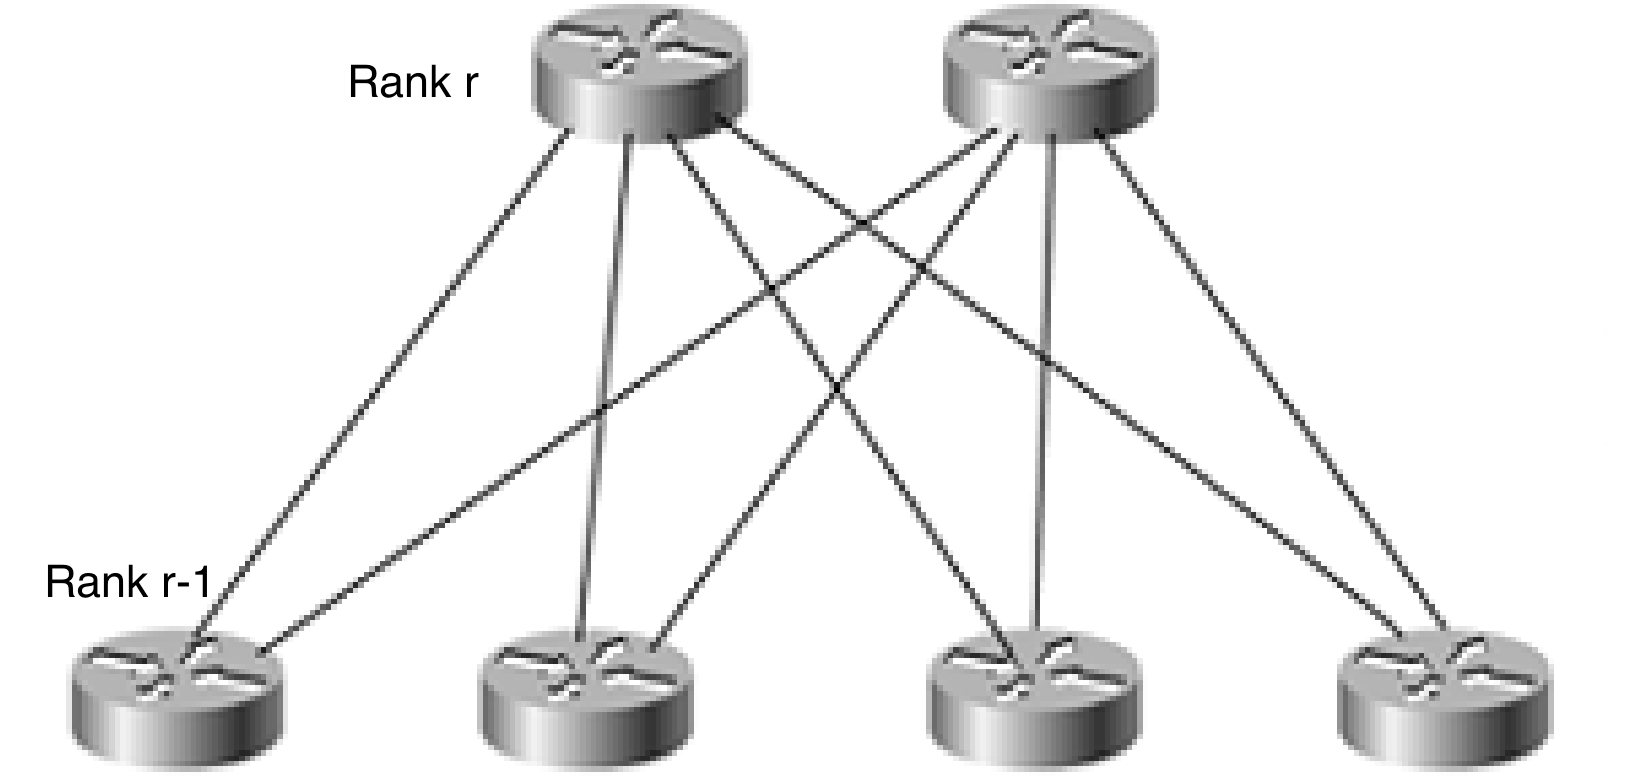
\includegraphics[width=8cm]{Designing_a_network_topology-M_H_Abu-Amara}
\caption{Hierarchical Mesh topology. Original from M.H.Abu-Amara$^3$} %make sure to update this footnote maually
\end{figure}

We close the chapter by expressing the above ideas using terminology from previous motivations mentioned in the Constellation whitepaper. 

If we consider each SOE as a basis of given rank $r$ in the space of the data dependency graph, we can calculate this volume as the integral over the outer product space of these basis, which is a differential r-form.
The notion of volume of space of the nodes across ranks $1$ through $r$ is
{$\int_\mathcal{M} \epsilon_1 \wedge \dots \wedge \epsilon_r.$}
Here $\mathcal{M}$ is a manifold and $\epsilon_r$ is a basis of the vector space of rank $r$. 
Each collection in the data dependency graph has the basis and rank of the node that emitted it. Within our model this would be explicitly defined as the numerical integration over the outer product of our cohomological definition
\footnote{Blockchain cohomology text\\ https://arxiv.org/abs/1805.07047},
which is a vector space given by the tensor product of each space across ranks 
{$\sum_{1 \dots r} \Gamma^{\epsilon_1} \otimes \dots \otimes \Gamma^{\epsilon_r}$}.
Each $\Gamma^{\epsilon_i}$ is a manifold corresponding to a rank in the differential form above, subordinate to the rank before it. If we assume a uniform data transmission, we can define bandwidth in SOE/s as the total space
\footnote{ftp.cis.upenn text on diff. geo., see sec 9.2\\ \url{ftp.cis.upenn.edu/pub/cis610/public_html/diffgeom4.pdf}} 
of the resources given by each node
\begin{equation*} \label{eq2}
\begin{split}
B_{\mathrm{SOE}/\mathrm{s}} = \sum_{i\,\in\,\{1, \dots, r\}} \int \rho_i\, \theta_i\, \omega,
\end{split}
\end{equation*}
where $\rho_i$ is a partition of unity and $\theta_i$ is a discrete diffeomorphism on our spaces $r$-form, $\omega$. This amounts to the effect that the protocol has on the total configuration space.
We determine a measure of performance, by mapping each entry in the bandwidth space to its normalized Shannon entropy, giving us a measure of relative information gain:
\begin{equation*} \label{eq3}
\begin{split}
B_\mathrm{Entropy} = \sum_{i\,\in\,\{1, \dots, r\}} \int \rho_i\, H_i\, \omega.
\end{split}
\end{equation*}
Here 
{$H_i(p) = - \tfrac{1}{\log_b(i)} \sum_j p_j \log_b(p_j)$}
is the normalized Shannon entropy, where $p$ is a discrete probability measure of how the result of a node's actions deviate from the acceptable state of the protocol and $b$ is our base. The later is binary, as we deal with bits. Reduction in entropy can be seen as a measure of efficiency. Normalized entropy is advantageous as it scales with sample size and has shown effective at anomaly detection in networks
\footnote{Karthik, P. ``Detecting Anomalies Based On Entropy-Estimation''\\ \url{http://ijsetr.org/wp-content/uploads/2013/07/IJSETR-VOL-2-ISSUE-4-910-915.pdf}}.

\section{Summary and Outlook}
The Constellation validator rewards model forms a well defined feature space for defining a reputation model, which is core to reputation based consensus. Facilitator selection is governed by this model which optimizes the network topology bases on the performance of each node. By tying optimal network organization to the criteria for facilitator selection, such a model embodies the adaptive qualities of a Generative economic model.

In addition to forming a tractable kernel for a reputation model based on performance, defining our dynamics in terms of a differential model allows for econometric methods like equilibria analysis to be employed. This enables analysis of the stability of our model under attacks or an influx of \$DAG used to pay for transactions. Equilibria analysis of this model will the a topic of future work.

\bibliographystyle{plain}
\end{document}
